\section{Global Memory - cudaMemcpy} 
\subsection{cudaMemcpy Task}

In this Task, the use of cudaMalloc(\&hmem, dat); and cudaMemcpy(hmem, dmem, dat, cudaMemcpyDeviceToDevice); was analyzed. That way we copy data from device to device. In the Graph \ref{fig:exc03_1_D2D} we can see, that a saturation of the coppying speed occurs on higher data transportation rates. In our Graph, we also show the other coppying speed of the other data. If you would like to take a look at our data, the data of the graphs is in folder (\url{exc03/Latex_File/data/analysis}).

\begin{figure}[H]
    \centering
    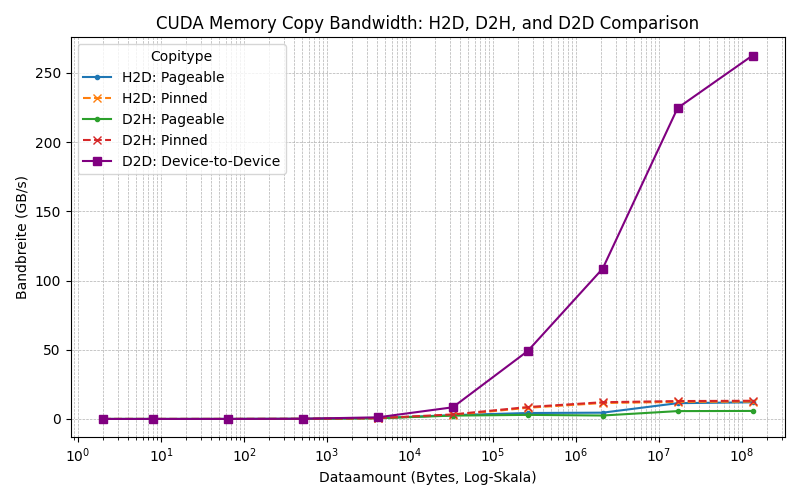
\includegraphics[width=1\textwidth]{pictures/exc03_1_D2D_together.png}
    \caption{Speed difference of Device to Device memory copy}
    \label{fig:exc03_1_D2D}
\end{figure}